%_____________________________________________________________________________________________ 
% LATEX Template: Department of Comp/IT BTech Project Reports
% Main Report
% Sun Apr 1 20:40:00 IST 2011
% 
%_____________________________________________________________________________________________ 

\documentclass[a4paper,14pt,onecolumn]{report}

%_____________________________________________________________________________________________ 
% Inclusion of Required Packages
%_____________________________________________________________________________________________ 
\usepackage[dvips]{graphics}
\usepackage{color}
\usepackage{epsfig}
\usepackage{longtable}
%_____________________________________________________________________________________________ 
% Page Layout
%_____________________________________________________________________________________________ 
\setlength{\textwidth}{6.27in}
\setlength{\textheight}{9.69in}
\setlength{\topmargin}{0.0in}
\setlength{\oddsidemargin}{0.0in}			% Customisable
\setlength{\headheight}{0.0in}
\setlength{\headsep}{0.0in}
\setlength{\topskip}{0.0in}
%_____________________________________________________________________________________________ 
% Font Definition
%_____________________________________________________________________________________________ 
\fontencoding{T1}		% Font specification : Times New Roman, Bold, Normal, 18
\fontfamily{cmr}		% Roman
\fontseries{m}			% Medium
\fontshape{n}			% Upright
\fontsize{14pt}{5}		
\linespread{1.5}		% Vertical spacing between lines
\selectfont			% Select the specified font
%_____________________________________________________________________________________________ 
% Main report starts here
%_____________________________________________________________________________________________ 

\begin{document}	% Start of Report
%_____________________________________________________________________________________________ 
\pagestyle{empty}
%_____________________________________________________________________________________________ 
% A Holistic Approach to Autonomic Self-Healing Cloud Computing Architecture
% Title Page
% Fri Apr 19 12:50:42 IST 2013
%___________________________________________
\DeclareGraphicsExtensions{.png, .ps, .jpg}
\begin{titlepage}
\begin{center}
\LARGE{\bf{A HOLISTIC APPROACH TO AUTONOMIC SELF-HEALING CLOUD COMPUTING ARCHITECTURE\\}}	% LARGE = 17.28
\vspace{10pt}
\Large{\bf{A Project Report\\}}		% Large = 14.40
\Large{\em{Submitted by\\}}
\begin{table}[htbp]
	\begin{center}
	\begin{tabular}{ l c c l }
	\Large\bf{Abhishek Kalpesh Bhavsar} & & & \Large\bf{110903064} \\[0.3cm] 
	\Large\bf{Ameya Ajit More} & & & \Large\bf{110903049} \\[0.3cm] 
	\Large\bf{Chinmay Sanjay Kulkarni} & & & \Large\bf{110903067} \\[0.3cm] 
	\Large\bf{Dheeraj Prakash Oswal} & & & \Large\bf{141003069} \\
	\end{tabular}
	\end{center}
	\end{table}
\Large{\em{in partial fulfilment for the award of the degree\\ \vspace{1.5pt}of\\}}
\LARGE{\bf{B.Tech Computer Engineering\\}}% Mention only appropriate degree.
\vspace{20pt}
%names of advisors
\Large{Under the guidance of\\ }
\Large{\bf{Dr. J. V. Aghav}\\}
\Large{College of Engineering, Pune\\}
\vspace{10pt}
%coep logo added
\begin{figure}[h]
\centering

\includegraphics[width=3cm,height=3cm]{figures/coeplogo.eps}
\end{figure}
\Large{\bf{DEPARTMENT OF COMPUTER ENGINEERING AND \\INFORMATION TECHNOLOGY,\\ 
COLLEGE OF ENGINEERING, PUNE-5}}
\vfill
\large{April, 2013}
\end{center}
\end{titlepage}

%\maketitle			% *Generate* the defined title. No definition - no gereration

%_____________________________________________________________________________________________ 
% LATEX Template: Department of Comp/IT BTech Project Reports
% Certificate Page
% Sun Mar 27 10:25:35 IST 2011
% 
% Note: UK English spellings used. 
%_____________________________________________________________________________________________ 
\thispagestyle{empty}
\linespread{2}
\begin{center}			% LARGE = 18
	\Large{\bf{DEPARTMENT OF COMPUTER ENGINEERING AND\\  INFORMATION TECHNOLOGY,\\ 
	       COLLEGE OF ENGINEERING, PUNE\\}}	
\end{center}

\vspace{20pt}			% Vertical space between dept name and ``certi''

\begin{center}
	\Large{\bf{CERTIFICATE\\}}
\end{center}

\vspace{20pt}

\linespread{2}			% Double spacing between lines
\selectfont
\large{
Certified that this project, titled ``A HOLISTIC APPROACH TO AUTONOMIC SELF-HEALING CLOUD COMPUTING ARCHITECTURE''
has been successfully completed by \\ 
\begin{table}[htbp]
	\begin{center}
	\begin{tabular}{ l c c l }
	\Large\bf{Abhishek Kalpesh Bhavsar} & & & \Large\bf{110903064} \\[0.3cm] 
	\Large\bf{Ameya Ajit More} & & & \Large\bf{110903049} \\[0.3cm] 
	\Large\bf{Chinmay Sanjay Kulkarni} & & & \Large\bf{110903067} \\[0.3cm] 
	\Large\bf{Dheeraj Prakash Oswal} & & & \Large\bf{141003069} \\
	\end{tabular}
	\end{center}
	\end{table} \\
and is approved for the partial fulfilment of the requirements for the degree of 
``B.Tech. Computer Engineering''.
}

\vspace{20pt}

\begin{center}		% Horizontal spacing used to keep the signatures in columns at the ends of
			% lines

SIGNATURE\hspace{\stretch{1}}SIGNATURE\\
\normalsize{\bf{DR. J. V. AGHAV\hspace{\stretch{1}}DR. J. V. AGHAV\\
Project Guide\hspace{\stretch{1}}Head}\\
Department of Computer Engineering\hspace{\stretch{1}}Department of Computer Engineering\\
and Information Technology,\hspace{\stretch{1}}and Information Technology,\\
College of Engineering Pune,\hspace{\stretch{1}}College of Engineering Pune,\\
Shivajinagar, Pune - 5.\hspace{\stretch{1}}Shivajinagar, Pune - 5.}
\end{center}

		% Certificate page will come here. But its been typeset 
				% independently in certi.tex

%_____________________________________________________________________________________________ 
% A Holistic Approach to Autonomic Self-Healing Cloud Computing Architecture
% Abstract Page
% Fri Apr 19 12:50:42 IST 2013
%___________________________________________
\begin{abstract}
%\addcontentsline{toc}{chapter}{Abstract}	% This makes sure abstract is included in contents.
Cloud computing systems are prone to errors and faults and a major amount of task is wasted in maintaining the system and bring it back to a stable state after a fault. This maintenance currently is handled by human resources in the cloud computing architecture. Despite the emergence of ultra-reliable components, failure in cloud computing systems is still an unmitigated problem. As a result of this a lot of resources in the form of money and manpower and efforts in the form of man months is wasted. The proposed mechanism focuses efforts to make a cloud computing environment reliable and robust by proposing an autonomic, self healing architecture. We adopt a holistic approach to the problem and aim at proposing an architecture that is general enough to be adopted by a wide range of existing systems. Some of the major challenges include selecting the appropriate actions for healing and reducing the overhead thus making healing lightweight and transparent, yet effective. The proposed system architecture makes use of data mining techniques to generate rules based on gathered system data from logs. The rules are used to make decisions of corrective action and hence carry out the self-healing mechanism.
%Missing wikipedia citation.
\end{abstract}
%_____________________________________________________________________________________________ 
		% Absract: Independently typeset in file abstract.tex

\thispagestyle{empty}
\tableofcontents		% *Generate* the table of contents. No content - no table
				% LATEX needs to run 2-3 times over source to get this correct

\pagenumbering{roman}		% Lowercase roman numbering for prelim sections
\listoftables
\addcontentsline{toc}{chapter}{List of Tables}

\listoffigures
\addcontentsline{toc}{chapter}{List of Figures}

%\chapter*{List of Symbols}
%\addcontentsline{toc}{chapter}{List of Symbols}

\newpage
\pagenumbering{arabic}		% Change to Arabic numbers for main chapters.

%_____________________________________________________________________________________________ 
% A Holistic Approach to Autonomic Self-Healing Cloud Computing Architecture
% Chapter 1 - Introduction
% Fri Apr 19 12:50:42 IST 2013
%_____________________________________________________________________________________________ 

\chapter{Introduction}
The advent of computers kicked off a race for development of a unified computing platform that could provide for a centralized computing facility, large and reliable storage and increased accessibility. This race brought about revolutionary technologies like Grid Computing, Clustered Systems, Distributed System and many others. Cloud Computing is the most recent development in this field and shows a lot of promise.
\section{Cloud Computing}
Cloud computing is a framework that revolves around the concept of providing services such as network storage and computational capabilities. One of the major motivations behind the development of cloud computing was to provide the above mentioned capabilities without the need to physically possess the resources. This is important as it makes available the resources even to individuals that may not possess the strength to set up the infrastructure needed to deliver such a computational environment. Users could thus avail services on subscription through service providers such as Google, Amazon etc.

Services provided by the cloud need not be only of the form of software servers, rather individuals could subscribe to an entire computing infrastructure. We illustrate further, the different services provided by the cloud-computing environment.
\subsection{Infrastructure as a Service}
Infrastructure as a Service aims at outsourcing hardware resources such as computational power, network and storage. This means that an individual can access the hardware resources as his own but it is the service provider who assumes the responsibility of setting up, maintaining and housing it. Some of the major Infrastructures available for subscription are
	\begin{itemize}
		\item Virtual Machines
		\item Servers
		\item Storage
		\item Network
	\end{itemize}
It should be noted that though all these infrastructural facilities are provided to the user as a whole, they might be distributed over various areas, even geographically separated.
\subsection{Platform as a Service}
Platform as a Service is a service model that provides a solution stack as a service. The service provider provides an individual a set of tools to develop and deploy software. PaaS allows individuals to build multi-tenant applications that can be concurrently accessed by a lot of users. PaaS provides subscription for
	\begin{itemize}
		\item Execution Runtime
		\item Database
		\item Web-server
		\item Development Tools
	\end{itemize}
\subsection{Software as a Service}
Software as a Service allows the software and its data to be placed on a remote server i.e. the cloud. SaaS allows this software by a subscriber using a remote machine like a desktop terminal via a web browser. Softwares that can be hosted on a cloud are
	\begin{itemize}
		\item Customer Relationship Management
		\item Management Information Systems
		\item Human Resource Management
		\item Enterprise Resource Planning
		\item Content Management
		\item Email
		\item Virtual Desktop
	\end{itemize}

\section{Motivation}
There is an ever-increasing demand for large-scale cloud computing systems with tens to hundreds of thousands of computing nodes that are being designed and deployed. The large scale of cloud computing environments, combined with the ever-growing system complexity, has made reliability a tremendous challenge. Component reliability becomes more difficult with the increasing complexity of the cloud components as well as growing system size.\cite{FAILURE_3} In order to improve component reliability, considerable research has been done to make cloud computing architectures resilient to faults and to make their applications more robust. The main aim is to create a self-healing cloud architecture that can efficiently detect failures in the system and take the corrective action based on meta-learning techniques.

\section{Main Contribution}
In this study, we propose a dynamic meta-learning architecture that can detect possible failures in the cloud computing system. These failures are detected with reasonable prediction accuracy on the basis of failure logs over a large period of time. The architecture consists of two basic parts to predict and take corrective action:
	\begin{itemize}
		\item Part one preprocesses and analyzes system event logs. The preprocessed (scrubbed) data is analyzed by means of association rule based machine learning to examine interesting events that may possibly lead to faults. The machine learning techniques are also used to identify failure patterns amongst the different cloud components.
		\item Part two uses the rules generated by the first part in order to carry out the corrective action and hence prevent failure. This may be done by means of migrating virtual machines running on computing nodes that are predicted to fail to another computing node.
	\end{itemize}
%These two parts, along with their main components, are illustrated in (*******FIG NUMBER*******). The details of the main components will be described in (****Section no.****).
% Insert cross reference to figure number and section.
%_____________________________________________________________________________________________ 

		% Add each chapter here in this fashion.
				% No need to write all font and page specs in the chapter
				% files. There only typesetting tags are required.
%_____________________________________________________________________________________________ 
% A Holistic Approach to Autonomic Self-Healing Cloud Computing Architecture
% Chapter 2 - 
% Fri Apr 19 12:50:42 IST 2013
%_____________________________________________________________________________________________ 

\chapter{Layered Architecture of a Cloud Computing Environment}
A Cloud Computing Environment can be looked upon from the perspective of a layered architecture as divided into 8 layers each interlinked with the layers above and below it and divided into 3 major parts.
\section{Supporting (IT) Infrastructure}
This layer houses all the actual resources and computing power of the entire system. This layer if of not much importance from the perspective of building autonomic system in a cloud, as it is hardware dependent and a lot of work is already done in this layer.
\section{Cloud Specific Infrastructure}
This is the layer that provides most scope for work and it is the only layer that actually defines the cloud-computing environment. 
\subsection{Cloud (Web) applications}
This layer includes the services and APIs written using programming platforms like Java, PHP, and Silverlight etc. Making changes to this layer is not feasible because it would mean putting additional burden on the programmers to design systems to incorporate autonomic computing and would make existing systems difficult to port. Also the motive behind the project is to provide a transparent mechanism for self-healing and autonomic computing that cannot be provided through this.
\subsection{Cloud Software Environment}
This is the layer that defines the cloud-computing environment. It makes use of the layers below to provide a unified computing environment in the form of a cloud. This is the layer where the Platform-as-a-Service and Infrastructure-as-a-Service frameworks of the cloud reside.
The cloud software infrastructure layer provides an abstraction level for basic IT resources that are offered as services to higher layers:
	\begin{itemize}
		\item Computational resources (usually VMEs)
		\item Storage
		\item (Network) communication
	\end{itemize}
These services can be used individually, as is typically the case with storage services, but they’re often bundled such that servers are delivered with certain network connectivity and (often) access to storage. This bundle, with or without storage, is usually referred to as IaaS.
The cloud software environment layer provides services at the application platform level: 
	\begin{itemize}
		\item A development and runtime environment for services and applications written in one or more supported languages
		\item Storage services (a database interface rather than file share)
		\item Communication infrastructure, such as Microsoft’s Azure service bus.
	\end{itemize}
\subsubsection{Computational Resources}
The cloud-computing environment provides a set of computing resources that can be used to perform work that is desired.
\subsubsection{Storage}
One of the major resources that a cloud provides is storage on demand.
\subsubsection{Communication}
The backbone of the entire cloud-computing environment is the communication network that binds various nodes.
We propose that the solution be planned in regard to managing this layer efficiently to provide a robust, self-healing, autonomic cloud-computing system that is fault tolerant and exhibits capabilities to resist and resolve future failures thus making the system impervious to faults.

\subsection{Service Customer}
This is the highest layer of abstraction that hides all the details of the lower layer and provides services that makes use of the lower layers to do actual work. The layer houses the front end and other network services involved in delivering the services to the end user and actual transmission of data between different components of a cloud computing environment.
The layer is a very high level abstraction of the layers below it and does not provide opportunity directly for building an autonomic computing environment. At the most, this layer can be used as an interface to provide interaction with the lower level.

%_____________________________________________________________________________________________ 

%_____________________________________________________________________________________________ 
% A Holistic Approach to Autonomic Self-Healing Cloud Computing Architecture
% Chapter 2 - 
% Fri Apr 19 12:50:42 IST 2013
%_____________________________________________________________________________________________

\chapter{Healing}
\section{Healing – An Overview}
Healing is the process of restoring a damaged or diseased system to its original working state, which is free from these problems. Being able to automatically detect and discover faults is of great importance for any healing system. The necessary actions must be taken in order to return to a working and fully functional working state. Cloud computing systems must also incorporate healing in order to ensure efficient working which can quickly, efficiently and accurately recover from a problematic state to its previous working state.  
The cloud computing environment can also suffer from a varied range of problems and failures. Some of these problems are 
	\begin{itemize}
		\item Security issues at both the client and at the server ends.
		\item Privacy of the users that have registered themselves with a remote cloud computing system.
		\item Integrity of the user data that is stored on the cloud servers.
		\item Theft of the user data stored on cloud servers.
		\item Loss of the user data stored on cloud servers.
		\item Applications to be stored on the cloud which are infected or are remotely stored on the cloud with malicious intent.
		\item The services and resources provided by a cloud computing infrastructure are not limited by geographic boundaries. The cloud computing systems provide these services to their clients through a single interface thus making it very difficult to locate the data of different users on the physical storage at the cloud server end.
	\end{itemize}
All the above-mentioned problems make it absolutely necessary to develop an efficient healing system for the cloud computing system.
% Citation needed for fault.
\section{Faults}
Any system that is working perfectly can be susceptible to a large number of faults. Depending on the tasks executed by that system, these faults may take a varied number of forms. The combined effect of these faults is a decrease in the productivity of the system and hence a drop in the system efficiency. In layman terms, the given system no longer functions as it used to before the occurence of the faults in the system. These faults may occur at different levels in the system architecture.
Furthermore, certain faults can trigger the occurence of subsequent faults and this can be disastrous.
A fault in a system is thus a malfunction, that leads to a ceratin deviation from the expected behavior of the system. If we consider the case of a system of inter-connected computers, faults may occur due to a large number of factors, including hardware failure, software bugs, software failure and network problems. 
Three types of faults are observed in a typical distributed system of computers:
	\begin{itemize}
		\item Transient faults
		\item These faults occur once and then disappear. For example, a network message doesn't reach its destination but does when the message is retransmitted after some period of time. 
		\item Intermittent faults
		\item Intermittent faults fault that are reoccurring. These are the most irritating of faults and occur mainly due to component failures or improper inter-component operation, like a loose connection.
		\item Permanent faults
		\item This type of failure is persistent and it will continue to exist as long as the faulty system component is repaired or even fully replaced in extreme cases. Examples of this fault are disk head crashes, software bugs, and burnt-out power supplies. 
It is thus essential for any system to incorporate techniques to resolve these faults as quickly and effectively as possible. In general, a fault tolerent system is what is required.
	\end{itemize}
\section{Fault Tolerance}
The basic approach to building fault tolerant systems is redundancy. Redundancy may be applied at several levels. 
\subsection{Information redundancy}
Information redundancy is used to provide fault tolerance by replicating or coding the data. For example, a Hamming code is used to provide extra bits in the data in order to recover a certain ratio of failed bits. Other important samples used to provide information redundancy are parity memory, ECC (Error Correcting Codes) memory and ECC codes on data blocks.
\subsection{Time redundancy}
Time redundancy achieves fault tolerance by performing an operation several times. Retransmissions in a reliable point-to-point and the use of timeouts along with group communication are examples of time redundancy. This form of redundancy is extensively useful in the presence of transient or intermittent faults. It is of no use with permanent faults. An example is the retransmission of TCP/TP packets. 
\subsection{Physical redundancy}
Physical redundancy deals with devices rather than data. Extra equipment is added to enable the system to tolerate the loss of some failed components. RAID disks and backup name servers are examples of physical redundancy. 
There are many challenges with regard to the implementation of fault tolerant architecute for any distributed system or autonomic computing system. Some of these challenges are:
	\begin{itemize}
		\item Implementation of autonomic fault tolerance techniques is required for multiple instances of any application that is running on the several virtual machines which are provided via the cloud computing infrastructure.
		\item Fault tolerant techniques must be developed which are integrated with the existing workflow scheduling algorithms that have been implemented for the underlying autonomic system.
		\item It is important that a great level of reliability and availability of multiple cloud computing providers with independent software stacks be ensured. 
		\item Autonomic fault tolerant methods must react in accurate synchronization among the various interacting clouds, otherwise the solution itself can lead to future faults in the system.
It is quite obvious that the techniques that can be developed for automatic fault tolerance are accompanied by a large number of limitations. In the foresight of various users(clients) registered with a cloud, requesting services, it is thus a great ordeal to ensure efficient provision of services without error. We cannot rely on fault tolerant mechanisms regardless of them being automatic.
	\end{itemize}
It is extremely difficult to synchronise fault repairs amongst the various inter-connected nodes of our autonomic cloud computing system, thus manual intervention in the healing process must be kept to a minimal level. Apart from synchronization, many other aspects must also be considered, including automatic and accurate load balancing in the unfortunate case of a the failure of a node or any component of the cloud server. It is this that has led to the growing demand for an autonomic cloud computing system that is capable of “self-healing”, keeping in mind that the system is not completely fault tolerant and impervious to faults.
\section{Need for Prediction}
The Cloud Computing environment is distributed over geographical locations. Also, inheritant in the definition of Cloud Computing, is the notion of leasing resources to third parties. The Cloud service provider needs to ensure uninterrupted and failure proof serivce. Thus the distributed nature and service liabilities entail a robust system which is reliable and requires minimum human intervention. One of the most fundamental and essential features that must be incorporated to achieve these goals is failure prediction. Failure prediction is an ensemble of various analytical techniques which work together closely to predict failures and thus trigger healing action.
\section{Self-Healing}
Ever since development of modern computers it has become very difficult to rectify the system faults and manage recovery from malicious attacks due to the increase in complexity of the systems. All these factors resulted in the study in the field of autonomic computing and have explored the concept of self-healing systems. Autonomic computing is a self-managing computing model named after, and patterned on, the human body's autonomic nervous system. Self-healing in autonomous computing is described as the process to to free people from discovering, recovering, and failures.  Self-healing systems are expected to heal themselves at runtime in response to any change in environment or operational circumstances. Thus, the goal of self-healing is to prevent disastrous failure through prompt execution of certain proposed actions. We need a self-healing mechanism which is expected to monitor, diagnose, recover from faults and regain normative performance levels independently. The Self-healing technology enhances the system reliability by removing the need for human operation, as human configuration and maintenance of complicated systems makes the system more vulnerable to errors.  Conventional ways to eliminate these errors would include log-based level, model-based level, and component-based level approaches. These approaches do support some parts of the self-healing process but not whole process which includes monitoring, filtering, translation, analysis, diagnosis, decision and healing.
%_____________________________________________________________________________________________
		
%_____________________________________________________________________________________________ 
% A Holistic Approach to Autonomic Self-Healing Cloud Computing Architecture
% Chapter 3 - Existing Solutions
% Fri Apr 19 12:53:32 IST 2013
%_____________________________________________________________________________________________
\chapter{Existing Solutions}
% Add Citation
\section{Autonomic computing system with model transfer}
\textbf{Patent number:} 7542956\cite{STRASSNER:2009}\\
Different data and commands are received from different devices and they are sent to an autonomic manager to produce a single normalized view of the information. The actual state is identified from the normalized view which is compared to the desired state. If there is a difference, configuration adjustment is done to reach the desired state.
	\begin{figure}[h]
		\begin{center}
			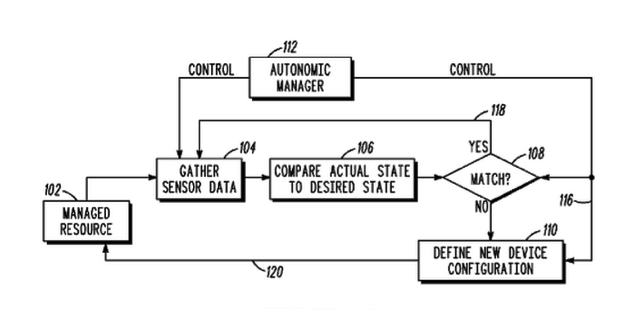
\includegraphics{figures/patent1_1.eps} 
			\caption{\small \sl Approach for Controlling a Managed Resource using an Autonomic System.\label{fig:Label1}} 
		\end{center} 
	\end{figure}

The technique uses machine learning, dependency processing and action determination logic to decide the action to be taken in case of a mismatch.
	\begin{figure}[h]
		\begin{center}
			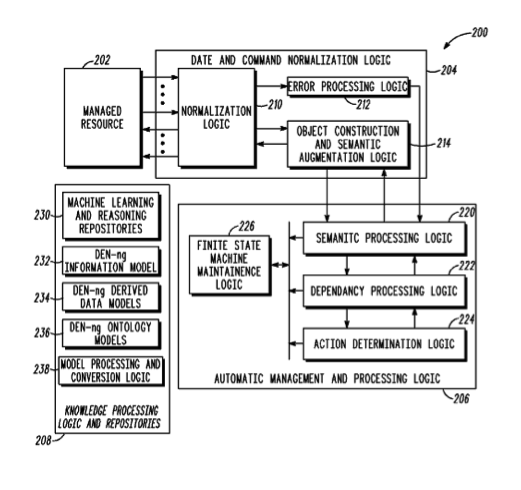
\includegraphics{figures/patent1_2.eps} 
			\caption{\small \sl Block diagram of an Autonomic System.\label{fig:Label2}} 
		\end{center} 
	\end{figure}
% Add Citation
\section{Architecture for a Self-Healing Computer System}
\textbf{Patent number:}  2010/0281134 (Patent pending)\cite{MELEN:2010}\\
The self healing system comprises a self healing processor and an error mitigation system, a code block associated with the operation of a portion of digital logic, dynamic signature analysis circuit. The processor executes the code block. The dynamic signature analysis circuit creates a dynamic signature representing the operation of the portion of digital logic associated with the code block. The error mitigation system receives the dynamic signature from the dynamic signature analysis circuit, and compares it with a static signature to determine if the signatures match. If the signatures do not match then the digital logic associated with the code block has an error. The error mitigation system retries execution of the code block. The error mitigation system stores log information describing the above events.
	\begin{figure}[h]
		\begin{center} 
			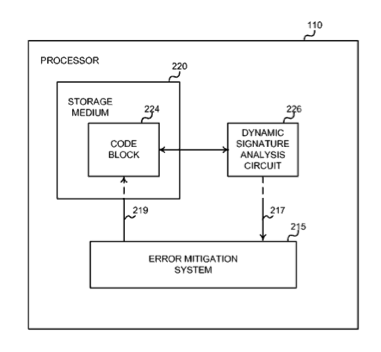
\includegraphics{figures/patent2_1.eps} 
			\caption{\small \sl Embodiment of a Self Healing Processor.\label{fig:Label3}} 
		\end{center} 
	\end{figure}

The Error Mitigation System is the core of the entire architecture. It houses a variety of components that help in finding out the error and correcting it. A lot of techniques like learning and lookup tables are used in this.
	\begin{figure}[h]
		\begin{center}
			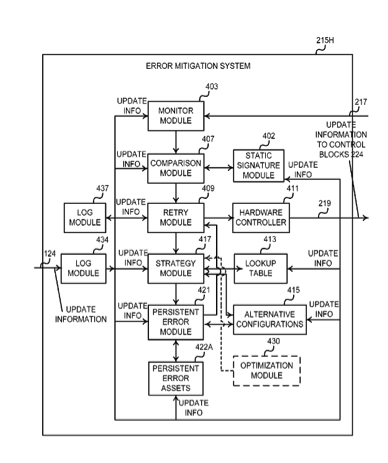
\includegraphics{figures/patent2_2.eps} 
			\caption{\small \sl Embodiment of an Error Mitigation System.\label{fig:Label4}} 
		\end{center} 
	\end{figure}

% Add Citation
\section{System and Method for Achieving Autonomic Computing Self Healing Utilizing Meta Level Reflection and Reasoning}
\textbf{Patent number:}  7260743\cite{FELLENSTEIN:2007}\\
In a base level a monitor detects an error in a production environment and provides reification message comprising data about the error to a meta level. A reasoning system in the meta level receives the reification message and analyzes the data using knowledge of computational components in the base level and identifies a self healing action for the error and returns a reversion message comprising a signal to implement the self healing action. Responsive to receiving the signal the base level implements the self-healing action.
	\begin{figure}[h]
		\begin{center}
			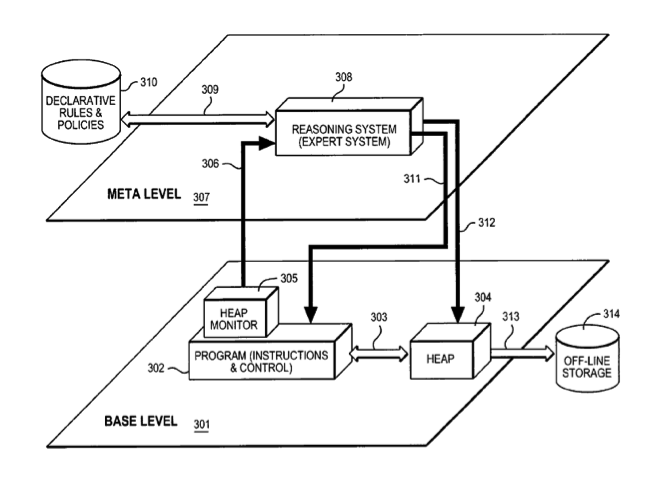
\includegraphics{figures/patent3.eps} 
			\caption{\small \sl System and method for Handling Errors.\label{fig:Label5}} 
		\end{center} 
	\end{figure}
\section{Comparison of the various approaches}
%\begin{table}		% Table
\begin{center}
\small		
%\begin{tabular}{| p{4cm} | p{4cm} | p{4cm} |}	% Format	
\begin{longtable}{| p{3cm} | p{3.5cm} | p{3.5cm} | p{3.5cm} |}
\hline 
\bf{Features} & \bf{Autonomic Computing System with Model Transfer } & \bf{Architecture for a Self Healing Computing System} & \bf{System and Method for Achieving Autonomic Computing Self Healing Utilising Meta Level Reflection and Reasoning}\\ \hline
{Comparison Parameters} & {Sensor State Comparison} & {Dynamic Signature Comparison} & {Reification Message} \\ \hline
{Separate Level used} & {No} & {No} & {Yes-Meta Level}\\ \hline
{Action Recommendation Logic} & {Learning based on creating models and mapping them to ontology includes semantic processing, dependency processing and action determination. } & {Static rules based. Uses Lookup table to map fault to strategy. Also has alternate configuration in case the basic strategy fails and a retry module. Strategy Optimisation is proposed not implemented.} & {Uses a reasoning system. Job is divided into two parts - detection (base level) and action recommendation (meta level). Transparency provided because of meta level.}\\ \hline
{Architecture specific requirements} & {Sensors} & {Error Mitigation System} & {Reasoning Expert System}\\ \hline
{Transparency} & {No} & {No} & {Yes- Multilevel}\\ \hline
{Feasibility} & {Excessive use of sensors. Too much of information collected, requires comparable hardware to process so much information.} & {Uses a specific processor that executes a code block and needs to interact with error mitigation system. Too much message passing} & {Meta level is idle most of the time. Fewer messages passed. Base level only sends messages when error is detected. Strategy can be easily decided and changed without modifications to the base level.}\\ \hline
{Dynamic Learning} & {Yes} & {No} & {Possible}\\ \hline
\caption{Comparison of the various approaches}
\end{longtable}
%\caption{A simple table: Test centuries}	% This will appear in List of Tables
\label{table1}
\end{center}
%\end{table}
%_____________________________________________________________________________________________ 


%_____________________________________________________________________________________________ 
% A Holistic Approach to Autonomic Self-Healing Cloud Computing Architecture
% Chapter 2 - 
% Fri Apr 19 12:50:42 IST 2013
%_____________________________________________________________________________________________

\chapter{Problem Statement}
\textit {``To provide a robust, self-healing, autonomic cloud-computing system that is fault tolerant and exhibits capabilities to resist and resolve future failures thus making the system impervious to faults."\\}
The project aims to come up with an architectural system that provides
	\begin{itemize}
		\item System to detect failures
		\item System to anticipate failures
		\item System to take necessary corrective actions once any of the above situation occurs
		\item Specifying inter-node communication
	\end{itemize}
%_____________________________________________________________________________________________

%_____________________________________________________________________________________________ 
% A Holistic Approach to Autonomic Self-Healing Cloud Computing Architecture
% Chapter 2 - 
% Fri Apr 19 12:50:42 IST 2013
%_____________________________________________________________________________________________
\chapter{Autonomic Self-Healing Architecture}
\section{Architecture Overview}
An autonomic mechanism will be used to deploy a monitoring system that will be responsible for collecting the resource utilization statistics of the remote hosts in the cloud. The collection of this data will be carried out periodically at regular intervals specified by the Autonomic Healing Engine. Each host will have a client version of the same monitoring system running as a daemon process. The client version of the monitoring system will send system resource utilization data to the monitoring system server application running on the Autonomic Healing Engine. The Autonomic Healing Engine passes this data to a Fault Detection Engine. The Fault Detection Engine is responsible for analyzing the data received and deducing the correct action to be taken in order to avoid the fault. The Fault Detection Engine stores statistical data such as load on the CPU, traffic on the Network Interface Cards of the various hosts, RAM usage, frequency of disk operations, etc. The Autonomic Healing Engine detects the Process Imprint of the executing process. An action deciding mechanism is implemented within the Fault Detection Engine that makes use of the Process Imprints and Process Association Graphs of the processes which are running on various instances of the hosts in the cloud.
	\begin{figure}[t]
		\begin{center}
			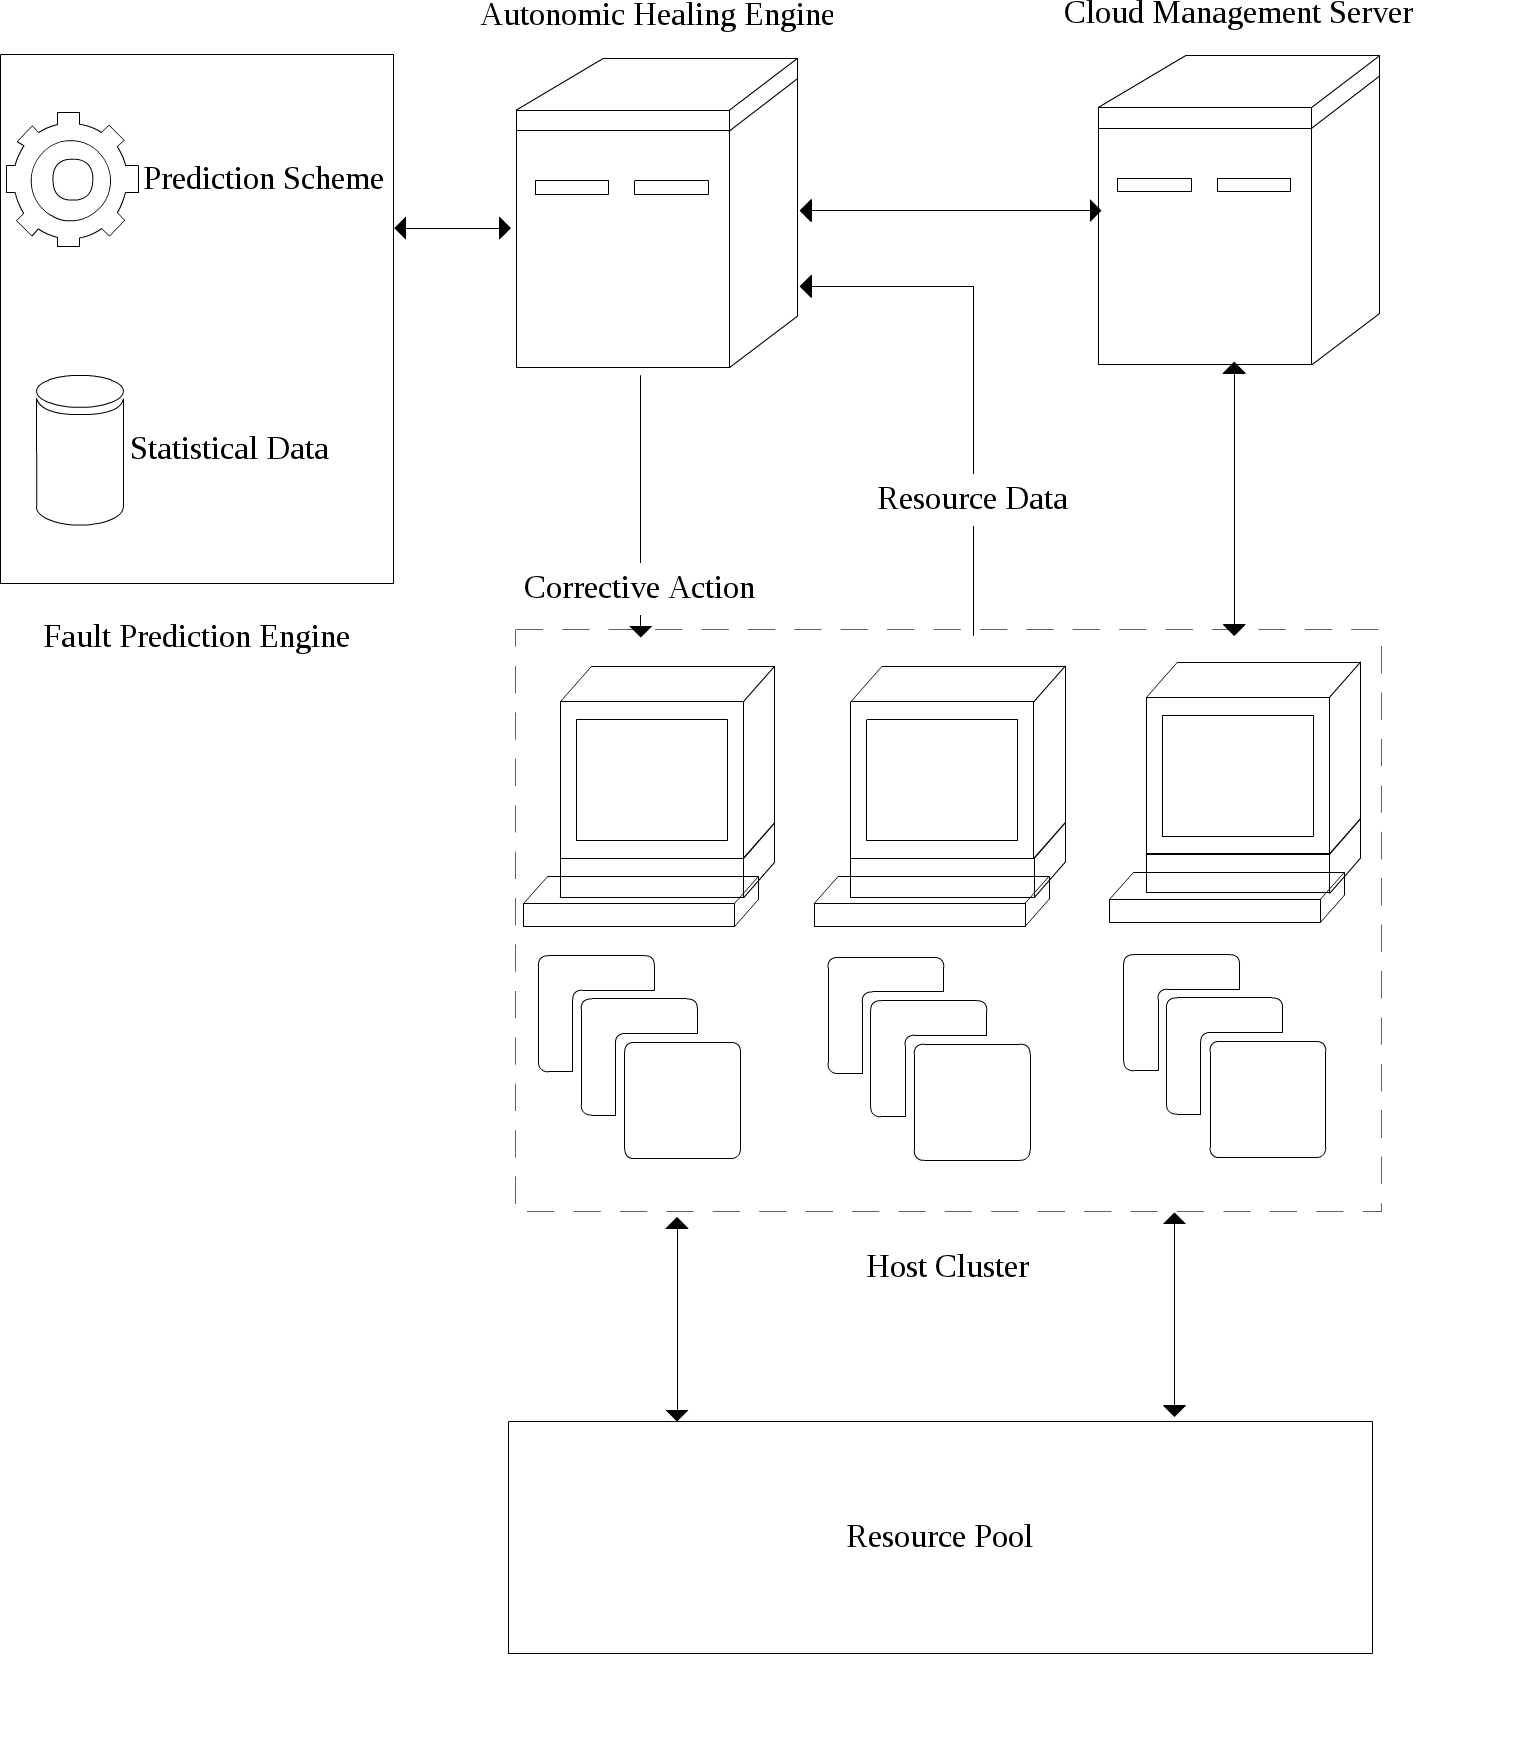
\includegraphics[width=10cm,height=10cm]{figures/cloud_architecture.eps} 
			\caption{\small \sl Autonomic Self-Healing Cloud Computing Architecture.\label{fig:Label6}} 
		\end{center} 
	\end{figure}
\section{Components}
\subsection{Resource Pool}
The Resource Pool consists of all the different resources that are allocated to the various virtual machines that are executing on the cloud host cluster. These resources include computational power, network bandwidth, memory, storage capacity, etc. The host cluster uses this resource pool to provide for the virtual machines that are running on them.
\subsection{Host Cluster}
This consists of all the compute units. This provides for all the computing power in the cloud. The hosts though independent, are managed by the cloud management server. The host powers all the Virtual Machines (VMs from here on) through their respective hypervisor. These VMs are directly accessible to users.

The hosts have a monitoring agent installed on them. This monitoring agent monitors the system and the log messages and forwards these log messages to the autonomic healing engine.
\subsection{Cloud Management Server}
The cloud management server powers the cloud. It is the backbone and acts as a link between hosts and resources. Cloud management server provides a unified view of the entire computing environment and also provides various management consoles for easy management.
\subsection{Autonomic Healing Engine}
The autonomic healing engine acts as a middleware between the host cluster and the fault prediction engine. It receives the system log messages from the hosts cluster and forwards them to the fault prediction engine for analysis and storage. The autonomic healing engine also receives the analyzed information from the fault prediction engine. This information then helps the autonomic healing engine to decide the action to be taken in case of a possible fault.

The separation from the fault prediction engine allows for pluggability. In essence, this means that the healing actions can be independent of the fault prediction scheme. The flexibility thus induced, helps to develop healing engines for an array of systems and thus makes the architecture truly holistic.
\subsection{Fault Prediction Engine}
The fault prediction engine analyses statistical data received from the autonomic healing engine. It uses data mining and machine learning techniques to recognize fault patterns and irregular behaviour in logs. It comprises of two parts
\subsubsection{Statistical Data}
This is the central data store that stores all previously analyzed results. This acts as the learning and training set for the prediction scheme. Storing of previous data helps in analyzing change of events and also patterns in change of types of failures overtime.
\subsubsection{Prediction Scheme}
The failure prediction scheme incorporates various data mining techniques to predict failures by generating rules. This module is independent of the autonomic healing engine and thus can be upgraded with new and better algorithms transparently.
\section{Prediction Scheme}
We now present a high level diagram of the proposed fault prediction scheme. The scheme involves two parts: data scrubbing and the other for fault prediction. We used the RAS logs from the Blue Gene/L System available at ANL.\cite{FAILURE_1}\cite{BLUEGENE_1}\cite{BLUEGENE_2}\cite{FAILURE_4} More information about the data can be found in the Appendix.
\begin{figure}[t]
		\begin{center}
			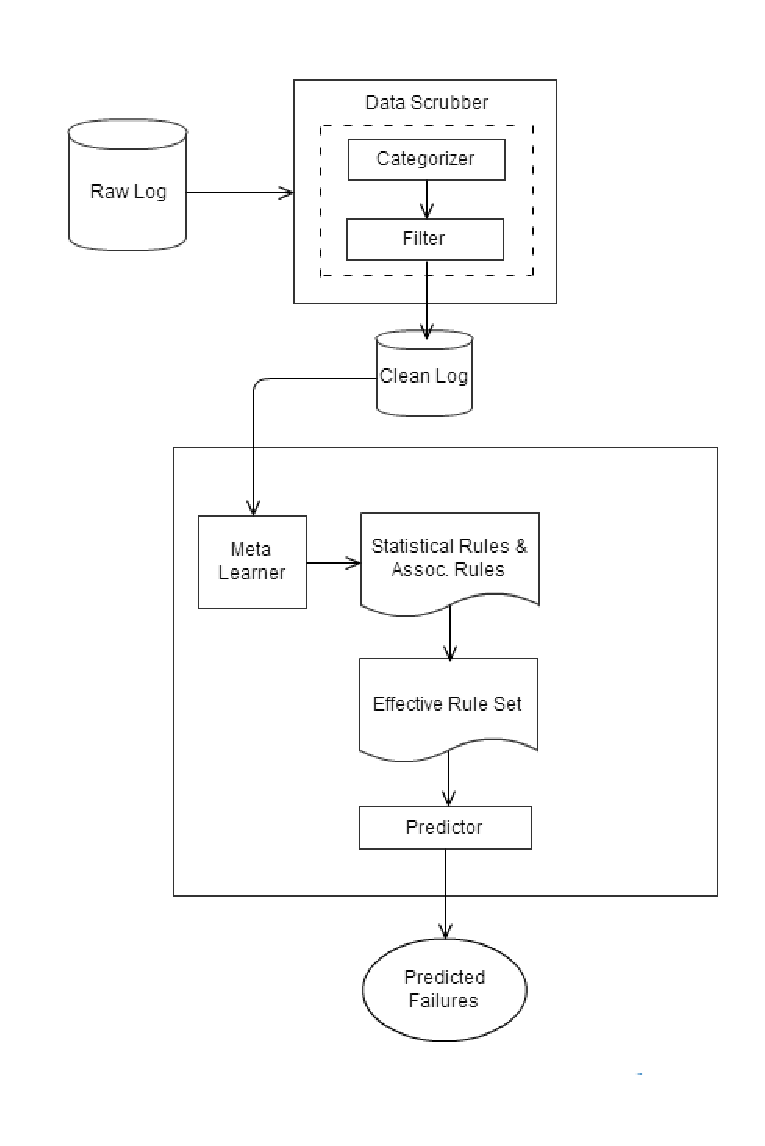
\includegraphics[width=10cm,height=10cm]{figures/failure_prediction_scheme.eps} 
			\caption{\small \sl Failure Prediction Scheme.\label{fig:Label7}} 
		\end{center} 
	\end{figure}

% Add cross reference.
\subsubsection{Data Scrubber}
The RAS logs cannot be used as is for data mining because of the unevenness in reporting the same type of error messages. The Data Scrubber handles all the actions of cleaning data so as to make it useable for mining. This steps also helps in reducing the amount of data storage space required to store the statistical data. Upon completion, the data scrubber intends to provide a list of unique events for failure prediction. This operation is further divided into two parts:
\paragraph{Event Categorization}
The RAS log, has a lot of information and because of the inherent distributed nature of the Blue Gene/L System, the logs cannot be used as is. The logs originate from a variety of different facilities and carry a lot of information that needs to be made meaningful to the data-mining program. We achieve this by categorizing events. Categorization of events maps the problem to a binary model where the particular event either occurs or not.

Event categorization is also done over the fatality of the event. This helps in recognizing failures efficiently.
\begin{figure}[t]
		\begin{center}
			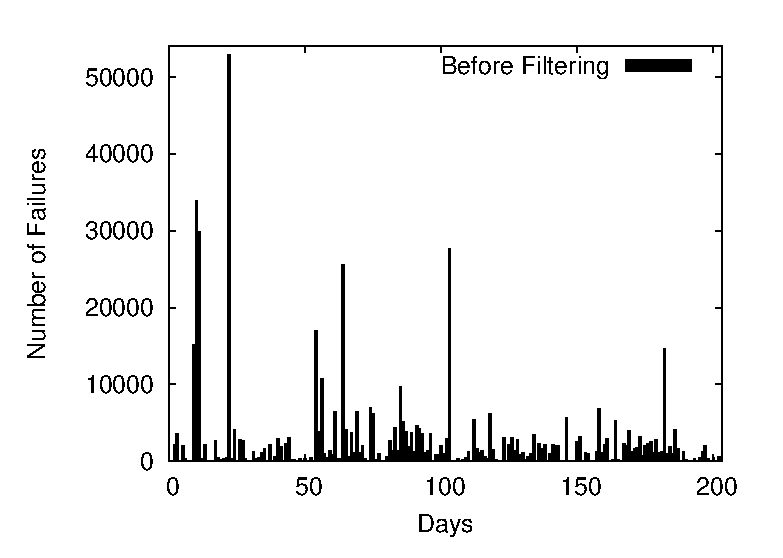
\includegraphics[width=10cm,height=7cm]{figures/histogram_unfiltered.eps} 
			\caption{\small \sl Number of failures per day before filtering\label{fig:Label7}} 
		\end{center} 
	\end{figure}
\paragraph{Event Filtering}
The distributed nature of the system causes a lot of duplication in the logs.\cite{SCRUBBING_1}\cite{FAILURE_2} As the job is distributed across nodes, the same job reports the same type of events multiple times. By studying event duplication times, we decided upon a 300 sec threshold for temporal compression of data. Event logs that appeared from the same location within a 300 sec window having the same category field were reported only once.


	\begin{figure}[b]
		\begin{center}
			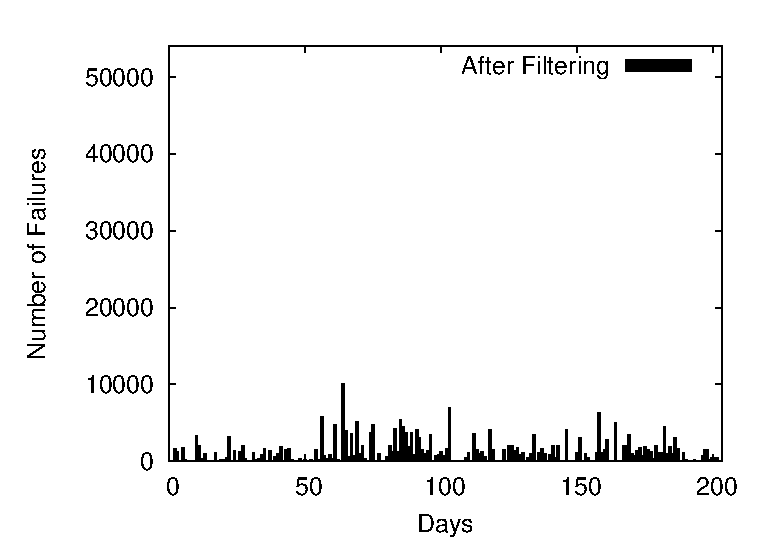
\includegraphics[width=10cm,height=7cm]{figures/histogram_filtered.eps} 
			\caption{\small \sl Number of failures per day after filtering\label{fig:Label7}} 
		\end{center} 
	\end{figure}


\subsection{Prediction}
The scrubbed data can now be processed by the Prediction Scheme mechanism in the Fault Prediction Engine, to analyze the data logs for failure patterns and irregular entries. The techniques of Association Rule Based Learning are used for this prediction. The scrubbed data logs are fed to the Weka Data Mining Tool.\cite{WEKA} Weka is configured to find associations amongst the entries in the data log. The Apriori algorithm is preferred to other Association Rule Based Learning algorithms because it can be easily configured to work with the large datasets that we must work with.\cite{APRIORI_1}\cite{APRIORI_2} We set the parameters of "Apriori Associate" to a minimum support of 0.01 and a threshold confidence value of 0.1. Once Weka has finished the processing of the data logs, it returns a set of rules. These rules are supplied with confidence values and those with high confidence values for failure events are predicted to be possible future failures. Those events that can lead to failures with a high confidence value trigger the Automatic Healing Engine to migrate VMs and their processes from this compute node that is likely to fail to a compute node that is processing normally.
%\begin{figure}[t]
%		\begin{center}
%			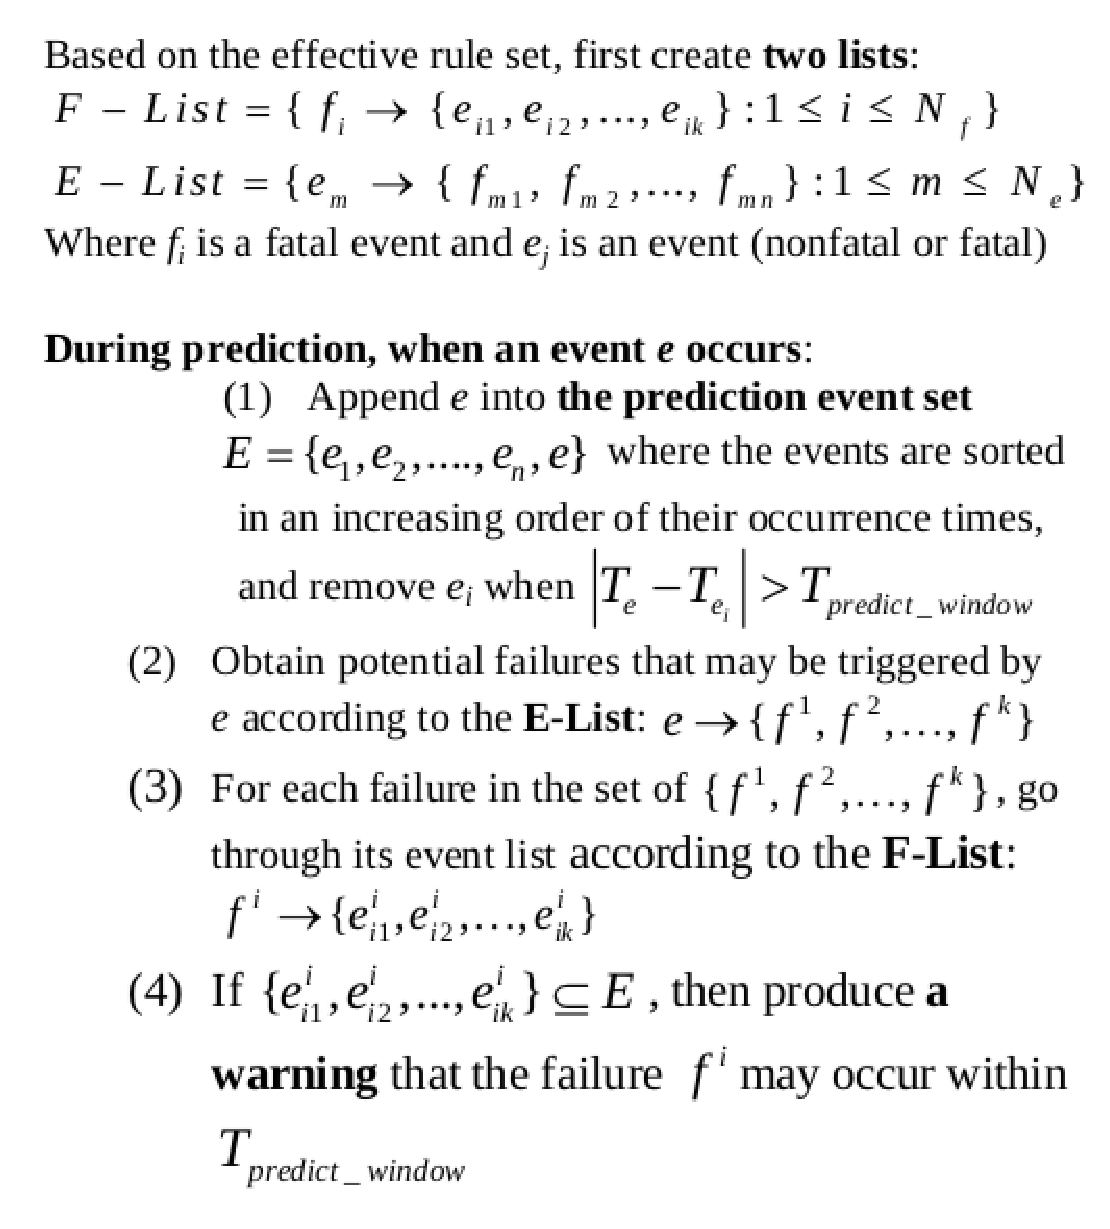
\includegraphics[width=8cm,height=10cm]{figures/prediction_algorithm.eps} 
%			\caption{\small \sl Prediction Algorithm.\label{fig:Label8}} 
%		\end{center} 
%	\end{figure}

\begin{algorithm}[b]
 \SetAlgoLined
% \KwData{
Based on the effective ruleset we first create two lists: \\ Triggered Failures List and Triggering Event List\\


 \begin{equation}
 	TE-List=\{f_i\rightarrow\{e_{i1}, e_{i2},\dots, e_{ik}\}:1 \le i\le N_f\}
 \end{equation}
 \begin{equation}
 	TF-List=\{e_m\rightarrow\{f_{m1}, f_{m2},\dots, f_{mn}\}:1 \le m \le N_e\}
 \end{equation}

 Where \begin{math}f_i\end{math} is a fatal event and \begin{math}e_j\end{math} is an event (nonfatal or fatal)

\textbf{During prediction, when an event e occurs}:
\begin{enumerate}
\item Append e into the prediction event set \begin{math}E=\{e_1,e_2,\dots,e_n,e\}\end{math} where the events are sorted in an increasing order of their occurence items, and remove \begin{math}e_i\end{math} when \begin{math}\mid T_e-T_{e_i}\mid>T_{predict\_window}\end{math}

\item Obtain potential failures that may be triggered by e according to the \begin{math}TF-List:e\rightarrow\{f_1, f_2,\dots,f_k\}\end{math}

\item For each failure in the set of \begin{math}\{f_1, f_2,\dots,f_k\}\end{math}, go through its event list according to the \begin{math}TE-List:f_i\rightarrow\{e_{i1}, e_{i2},\dots,e_{ik}\}\end{math}

\item If \begin{math}\{e_{i1}, e_{i2},\dots,e_{ik}\}\subseteq E\end{math}, then produce a warning that the failure \begin{math}f_i\end{math} may occur within \begin{math}T_{predict\_window}\end{math}

\end{enumerate}
% }
 

 \caption{Algorithm for Prediction}
\end{algorithm}


\appendix
\chapter{Overview of Blue Gene/L System}
The basic building block of the Blue Gene/L is called the computer chip. Each computer chip consists of two PPC 440 cores, with a 32 KB L1 cache and a 2 KB L2 cache. The cores share a 4 MB EDRAM L3 cache. A compute card contains two computer chips. A node card contains 16 compute cards, and a midplane holds 16 node cards with a total of 1024 processors. A midplane also contains several I/O nodes which are configured to handle file I/O and host communication. Each midplane also has one service card that performs system management services. These system management services include activitis such as monitoring node heartbeat and checking errors. 

In Blue Gene, the Cluster Monitoring and Control System (CMCS) service is implemented on the service nodes. The purpose of the CMCS is system monitoring and error checking. Specific device information is acquired by the service node, which is available on each midplane. This information includes RAS(reliability, availability and serviceability) events and other useful data, and is acquired by service nodes directly through the control network. A polling agent is used to collect runtime information from the computer and I/O nodes. This information is reported to the CMCS service, after which it is stored in a centralized DB2 repository. The granularity of this system event logging mechanism is less less than 1 ms.
\section{RAS Logs}
RAS stands for Rliability, Availability and Servicability. RAS logs are machine logs recorded by IBM machines and contain error traces and informational records . RAS logs have been commonly used for machine failure analysis. RAS messages for daemons that are down and jobs that are being rejected or vacated are always logged. The project uses RAS logs of the IBM Blue Gene/L machine recorded over six months to train the fault prediction mechanism and also to revise it. A sample RAS. A sample record from the Blue Gene/L RAS log is as follows:
\begin{table}[h]
\begin{center}
\small
\begin{tabular}{| p{1cm} | p{2.5cm} | p{1.5cm} | p{2cm} | c | c | p{3cm} |}
\hline	
	\bf{recid} & \bf{event\_time} & \bf{location} & \bf{event\_type} & \bf{facility} & \bf{severity} & \bf{entry\_data} \\ \hline
	1 & 2005-06-03-15.42.50.363779 & R02-M1-N0-C:J12-U11 & RAS & KERNEL & INFO & instruction cache parity error corrected \\ \hline
\end{tabular}
\label{table2}
\end{center}
	\caption{Sample Blue Gene/L RAS Log Entry.}
\end{table}
\begin{itemize}
	\item recid - Recid or record ID is used to uniquely identity a record in the RAS log.
	\item Location - Specifies the identifier used to identify the node card that reported the message.
	\item event\_type - Specifies the type of the event mostly RAS.
	\item Facility - Specifies the source from which the message originated.
	\item Severity - Specifies the severity of the message whether fatal, failure, non fatal informational message or severe.
	\item entry\_data - Specifies the actual message that was generated by the Blue Gene/L machine when the corresponding event occurred.
\end{itemize}

\chapter{Association Rule Learning}
In data mining, association rule learning is used for discovering interesting relations between variables in large databases. It is intended to identify strong rules discovered in databases using different measures of interestingness. 

The problem of association rule mining is defined as:\\
Let \begin{math}I=\{i_1, i_2,\ldots,i_n\}\end{math} be a set of \begin{math}n\end{math} binary attributes called ``items". Let \begin{math}D = \{t_1, t_2, \ldots, t_m\}\end{math} be a set of transactions called the ``database". Each transaction in \begin{math}D\end{math} has a unique transaction ID and contains a subset of the items in \begin{math}I\end{math}. A ``rule" is defined as an implication of the form \begin{math}X \Rightarrow Y\end{math} where \begin{math}X, Y \subseteq I\end{math} and \begin{math}X \cap Y = \emptyset\end{math}. The sets of items (for short ``itemsets") \begin{math}X\end{math} and \begin{math}Y\end{math} are called ``antecedent" (left-hand-side or LHS) and ``consequent" (right-hand-side or RHS) of the rule respectively.

\section{Useful Terms}
To select interesting rules from the set of all possible rules, constraints on various measures of significance and interest can be used. The best-known constraints are minimum thresholds on support and confidence.
	\begin{itemize}
		\item The ``support" \begin{math}\mathrm{supp}(X)\end{math} of an itemset \begin{math}X\end{math} is defined as the proportion of transactions in the data set which contain the itemset. 
		\item The ``confidence" of a rule is defined \begin{math}\mathrm{conf}(X\Rightarrow Y) = \mathrm{supp}(X \cup Y) / \mathrm{supp}(X)\end{math}. Here supp(X∪Y) means ``support for occurrences of transactions where `X and Y both' appear", not ``support for occurrences of transactions where `either X or Y appears'". Therefore, confidence is an estimate of the probability \begin{math}P(Y|X)\end{math}, the probability of finding the RHS of the rule in transactions under the condition that these transactions also contain the LHS.
		\item The ``lift" of a rule is defined as \begin{math} \mathrm{lift}(X\Rightarrow Y) = \frac{ \mathrm{supp}(X \cup Y)}{ \mathrm{supp}(X) \times \mathrm{supp}(Y) } \end{math} or the ratio of the observed support to that expected if X and Y were independent. 
		\item The ``conviction" of a rule is defined as \begin{math} \mathrm{conv}(X\Rightarrow Y) =\frac{ 1 - \mathrm{supp}(Y) }{ 1 - \mathrm{conf}(X\Rightarrow Y)}\end{math}. Thus, conviction can be interpreted as the ratio of the expected frequency that X occurs without Y (that is to say, the frequency that the rule makes an incorrect prediction) if X and Y were independent divided by the observed frequency of incorrect predictions.
	\end{itemize}
Association rules are usually required to satisfy a user-specified minimum support and a user-specified minimum confidence at the same time. Association rule generation is composed of two steps:
	\begin{enumerate}
		\item First, minimum support is applied to find all frequent itemsets in a database. 
		\item Second, these frequent itemsets and the minimum confidence constraint are used to form rules.
	\end{enumerate}
Apriori is the most efficient algorithm to mine association rules. It uses a breadth-first search strategy to count the support of itemsets and uses a candidate generation function to generate association rules.
\section{Apriori Algorithm for Association Rule Learning}
Apriori is an algorithm for frequent itemset mining. The Apriori Algorithm is used mainly for association rule learning over transactional databases. It proceeds by identifying the frequent individual items in the database and extending them to larger and larger item sets as long as those item sets appear sufficiently often in the database. The frequent item sets determined by Apriori can be used to determine association rules that highlight general trends in the database.

Apriori is designed to operate on databases containing transactions. Each transaction is seen as a set of items, which is called an ``itemset". Given a threshold \begin{math}C\end{math}, the Apriori algorithm identifies the itemsets which are subsets of at least \begin{math}C\end{math} transactions in the database. 

In the Candidate Generation Phase, the Apriori Algorithm uses a ``bottom up" approach, where frequent subsets are extended one item at a time, and groups of candidates are tested against the data. The algorithm terminates when no further successful extensions are found.
It generates candidate item sets of length \begin{math}k\end{math} from item sets of length \begin{math}k-1\end{math}.  Then it prunes the candidates that have an infrequent sub-pattern. Thus, the candidate set contains all frequent \begin{math}k\end{math}-length item sets. After that, it scans the transaction database to determine frequent item sets among the candidates.  

The pseudocode for the algorithm is given below for a transaction database \begin{math}T\end{math}, and a support threshold of \begin{math}\epsilon\end{math}. \begin{math}T\end{math} is a multiset and \begin{math}C_k\end{math} is the candidate set for level \begin{math}k\end{math}.  Generate() algorithm is assumed to generate the candidate sets from the large itemsets of the preceding level.

\indent \begin{math}\mathrm{Apriori}(T,\epsilon)\end{math}\\
\indent\indent \begin{math}L_1 \gets \{ \mathrm{large~1-itemsets} \} \end{math}\\
\indent\indent \begin{math}k \gets 2\end{math}\\
\indent\indent\indent \begin{math}\mathrm{\textbf{while}}~ L_{k-1} \neq \emptyset \end{math}\\
\indent\indent\indent\indent \begin{math}C_k \gets \{ c |c = a \cup \{b\}  \land  a \in L_{k-1} \land b \in \bigcup L_{k-1} \land b \not \in  a  \}\end{math}\\
\indent\indent\indent\indent \begin{math}\mathrm{\textbf{for}~transactions}~t \in T\end{math}\\
\indent\indent\indent\indent\indent \begin{math}C_t \gets \{ c | c \in C_k \land c \subseteq t \} \end{math}\\
\indent\indent\indent\indent\indent \begin{math}\mathrm{\textbf{for}~candidates}~c \in C_t\end{math}\\
\indent\indent\indent\indent\indent\indent \begin{math}count[c] \gets count[c]+1\end{math}\\
\indent\indent\indent\indent \begin{math}L_k \gets \{ c |c \in C_k \land ~ count[c] \geq \epsilon \}\end{math}\\
\indent\indent\indent\indent \begin{math}k \gets k+1\end{math}\\
\indent\indent\indent \begin{math}\mathrm{\textbf{return}}~\bigcup_k L_k\end{math}\\



\bibliographystyle{plain}  	  % You can change the style of writing bibliography.
\bibliography{coep_compit_report} % Instead of a .bib file, you can just write it in 
				  % a text file with \bibitem entries.
%_____________________________________________________________________________________________ 
\end{document}			% End of Report
